% --
% Master thesis main

\documentclass[twoside,openright]{scrreprt}
%\documentclass[report,mono,twoside,openright]{tugrazbooklet}
%\documentclass[a4paper]{book}

% added package prior to thesis
\usepackage[table]{xcolor}

% tu stuff
\usepackage[msc]{tugrazthesis}


% --
% bib

\usepackage[backend=biber,style=alphabetic]{biblatex}

% add my bib
\addbibresource{./bibl.bib}


% --
% my packages, macros and colors

% --
% added packages

% language packages (for quotes etc.)
\usepackage[ngerman, english]{babel}

% standard
\usepackage{array}
\usepackage{float}
\usepackage{tikz}
\usepackage{multirow}
\usepackage{amssymb}
\usepackage{amsmath}
\usepackage{amsfonts}
\usepackage{mathrsfs}
\usepackage{geometry}
\usepackage{graphicx}
\usepackage{subfigure}
\usepackage{rotating}
\usepackage{enumitem}
\usepackage{flafter}
\usepackage{psfrag}
\usepackage{wrapfig}

% float barrier
\usepackage{placeins}

% links
\usepackage[colorlinks=false, allcolors=blue]{hyperref}

% quotes language dependend
\usepackage[autostyle=true]{csquotes}

% SI units
\usepackage{siunitx}

% tables
\usepackage{booktabs}
\usepackage{caption}

% beautiful font and letters
\usepackage{yfonts}

% arbritrary font sizes (used for font size warning)
\usepackage{lmodern}

% float warning hack
\usepackage{scrhack}

% math stuff such as coloneqq
\usepackage{mathtools}

% ipa symbols
\usepackage{tipa}

% nice norm and abs symbols
\usepackage{physics}

% bold face symbold
\usepackage{bm}

% url and hyphenation for url
\usepackage{url}
\usepackage{xurl}

% hyphenation
\usepackage[htt]{hyphenat}


% --
% config of packages

% siunits
\sisetup{binary-units=true}
\sisetup{detect-all=true}
% --
% Macros

% text fromatting
\newcommand{\ditto}{---\texttt{"}---}

% refs
\newcommand{\rchp}[1]{Chapter~\ref{chp:#1}} 
\newcommand{\rchps}[1]{Chapters~\ref{chp:#1}} 
\newcommand{\rsec}[1]{Section~\ref{sec:#1}} 
\newcommand{\rsecs}[1]{Sections~\ref{sec:#1}} 
\newcommand{\rappendix}[1]{Appendix~\ref{#1}} 
\newcommand{\rfig}[1]{Figure~\ref{fig:#1}} 
\newcommand{\rfigs}[1]{Figures~\ref{fig:#1}} 
\newcommand{\rtab}[1]{Table~\ref{tab:#1}} 
\newcommand{\rtabs}[1]{Tables~\ref{tab:#1}} 
\newcommand{\rlst}[1]{Listing~\ref{lst:#1}} 
\newcommand{\rlsts}[1]{Listings.~\ref{lst:#1}}
\newcommand{\req}[1]{(\ref{eq:#1})}

% math
\newcommand{\R}{\mathbb{R}}
\newcommand{\N}{\mathbb{N}}
\newcommand{\E}{\mathbb{E}}
\newcommand{\C}{\mathbb{C}}
\newcommand{\lam}{\lambda}
\newcommand{\g}{\nabla}
\newcommand{\inner}[2]{\langle #1, #2\rangle}
\newcommand{\sign}[1]{\mathrm{sgn}(#1)}
\newcommand{\interior}{\mathrm{int}}
\newcommand{\domain}{\mathrm{dom}}
\newcommand{\gradx}[1]{\begin{pmatrix} \frac{\partial}{\partial #1_1}\\\vdots\\\frac{\partial}{\partial #1_n}\end{pmatrix}}
\newcommand{\partialx}[1]{\frac{\partial}{\partial x_{#1}}}
\newcommand{\ball}[1]{B_{\norm{\cdot}_\infty}[0, #1]}
\newcommand{\deltaBall}[1]{\delta_{B_{\norm{\cdot}_\infty}[0, #1]}}
\newcommand{\proxMap}[2]{\mathrm{prox}_{#1 #2}}
\newcommand{\mor}{\frac{1}{2 \lambda} \norm{x-y}^2}
\newcommand{\diag}[1]{\mathrm{diag(#1)\,}}
\newcommand{\id}{\mathrm{\,Id\,}}
\newcommand{\proj}[1]{\mathrm{proj}_{#1}}
\newcommand{\prox}[1]{\mathrm{prox}_{#1}}

% tables
\newcolumntype{M}[1]{>{\centering\arraybackslash}m{#1}}

% booktabs tables
\setlength{\heavyrulewidth}{1.5pt}
\setlength{\abovetopsep}{4pt}
% --
% colors


% unused
\definecolor{LightYellow}{HTML}{ffff99}

% thesis main color
\definecolor{ThesisColor}{HTML}{aabb99}

% thesis state color
\definecolor{grela}{RGB}{109, 199, 177}
\definecolor{yeola}{RGB}{217, 175, 107}
\definecolor{viola}{RGB}{185, 83,  126}


% --
% begin document

\begin{document}

% myself
\thesisauthor[Christian Walter]{Christian Walter, BSc}

% thesis title
\thesistitle[Short Thesis Title]{Key Word Spotting for Video Games\\with Neural Networks}

% Date of completion (optional argument sets a different \date{})
\thesisdate[ ]{Month Year}

% Supervisor headline (select male/female/plural version)
\supervisortitle{\germanenglish{Betreuerin/Betreuer}{Supervisor}}

% Supervisor info
\supervisor{Robert Legenstein, Univ.-Prof. Dipl.-Ing. Dr.techn.\\Institute of Theoretical Computer Science\\}

% Academic degree achieved with this thesis, according to your curriculum (check curriculum and select male/female version):
\academicdegree{Master of Science}

% curriculum
\curriculum{Individuelles Masterstudium}
%\curriculum{Information and Computer Engineering } % 411
%\curriculum{Computer Science } % 921


% --
% titles

% title page
\printthesistitle

% affidavit
\printaffidavit

% abstract en
\chapter*{Abstract}
Key Word Spotting is a branch of speech recognition and a valuable tool in the interaction between humans and machines in various situations. 
This thesis is specialised solely on the domain of Computer Games and analyzes possible scenarios of applications and challenges within. 
Especially the application of speech commands in triggering events in games is evaluated and discussed.

% abstract de
\chapter*{Kurzfassung}
% --
% deutscher abstract

Deutsche Kurzfassung der Abschlussarbeit
\cleardoublepage

% Acknowledgement
\chapter*{\germanenglish{Danksagung}{Acknowledgements}}
% --
% Acknowledgements

\chapter*{\germanenglish{Danksagung}{Acknowledgements}}
I am happy to thank all the people who helped and motivated me to create this master's thesis.
Great thanks belongs to my Supervisor Robert Legenstein without whom this thesis would not have been shaped to fit the likeness of an actual thesis.
Thank you for your fast and accurate responses, very valuable suggestions, and proof-reads.
Further, I would like to thank all my dear proof-readers for spending their free time in finding mistakes within this thesis.
Namely the proof-reader were: Simon Beck, Thomas Deppisch, Viktoria Fürst, Lisa Kerle, Thomas Rosenmeier, Jiwon Seo, Michael Walter, Tanja Walter, and Paavo Ylimys.
Also all contributors to the technical tools and packages used within this thesis are acknowledged, which certainly helped to finish this thesis within a mortal lifespan.
Further thanks goes to the creators of the speech commands dataset who published the dataset open access.
This saved me the effort of recording thousands of iterations of different keywords in order to play a video game with my own voice.
Finally, I would like to thank my family and friends for supporting me on this long journey during a really chaotic time.
Through all your help, it is now possible to confidently publish this thesis with a good conscience.
\cleardoublepage

% table of contents
\tableofcontents
\listoffigures
\listoftables

% acronyms
\chapter*{\germanenglish{Abk\"{u}rzungs- und Symbolverzeichnis}{List of Acronyms and Symbols}}
% --
% acronyms

\chapter*{\germanenglish{Abk\"{u}rzungs- und Symbolverzeichnis}{List of Acronyms and Symbols}}

\begin{tabular}{ l l }
% A
AR & Augmented Reality\\
ASR & Automatic Speech Recognition\\
AWGN & Additive White Gaussian Noise\\
% B
% C
CD & Compact Disc\\
CNN & Convolutional Neural Network\\
% D
D & Discriminator\\
DCGAN & Deep Convolutional Generative Adversarial Network\\
DCT & Discrete Cosine Transform\\
DFT & Discrete Fourier Transform\\
DNN & Deep Neural Network\\
DS-CNN & depth-wise separable Convolutional Neural Network\\
DTFT & Discrete-Time Fourier Transform\\
% E
EEG & Electroencephalogram\\
% F
FC & Fully-Connected\\
FFT & Fast Fourier Transform\\
FIFO & First In First Out\\
FPS & Frames Per Second\\
% G
G & Generator\\
GAN & Generative Adversarial Neural Network\\
% H
HMD & Head Mounted Device\\
HMM & Hidden Markov Model\\
% I
IPA & International Phonetic Alphabet\\
% J
% K
KWS & Key Word Spotting\\
% L
LSTM & Long Short Time Memory\\
% M
MFCC & Mel Frequency Cepstral Coefficients\\
% N
NAS & Neural Architecture Search\\
NLP & Natural Language Processing\\
% O
% P
PLP & Perceptual Linear Prediction\\
% Q
% R
ReLU & Rectified Linear Unit\\
RNN & Recurrent Neural Network\\
% S
SNR & Signal to Noise Ratio\\
STFT & Short-Time Fourier Transform\\
SVM & Support Vector Machine\\
% T
% U
% V
VR & Virtual Reality\\
% W
% X
% Y
% Z
\end{tabular}


% -- 
% content

% --
% Introduction

\chapter{Introduction}\label{sec:intro}
Controlling video games with the voice of a player in order to render certain actions within the game, is an interdisciplinary challenge between speech signal processing, machine learning and game design.
A microphone is required to capture the voice of a player providing a speech signal of a potential command for the video game.
The speech signal is usually extracted from raw audio samples to meaningful features, such as the Mel Frequency Cepstral Coefficients (MFCC) and being used as inputs to a Key Word Spotting (KWS) system with the task of classifying those features to the most probable command.
The spoken command should change states of specific game objects and therefore ideally enhance and extend the gaming experience of the players.
A simple schematic of the whole process is shown in \rfig{intro_kws}.
\begin{figure}[!ht]
  \centering
    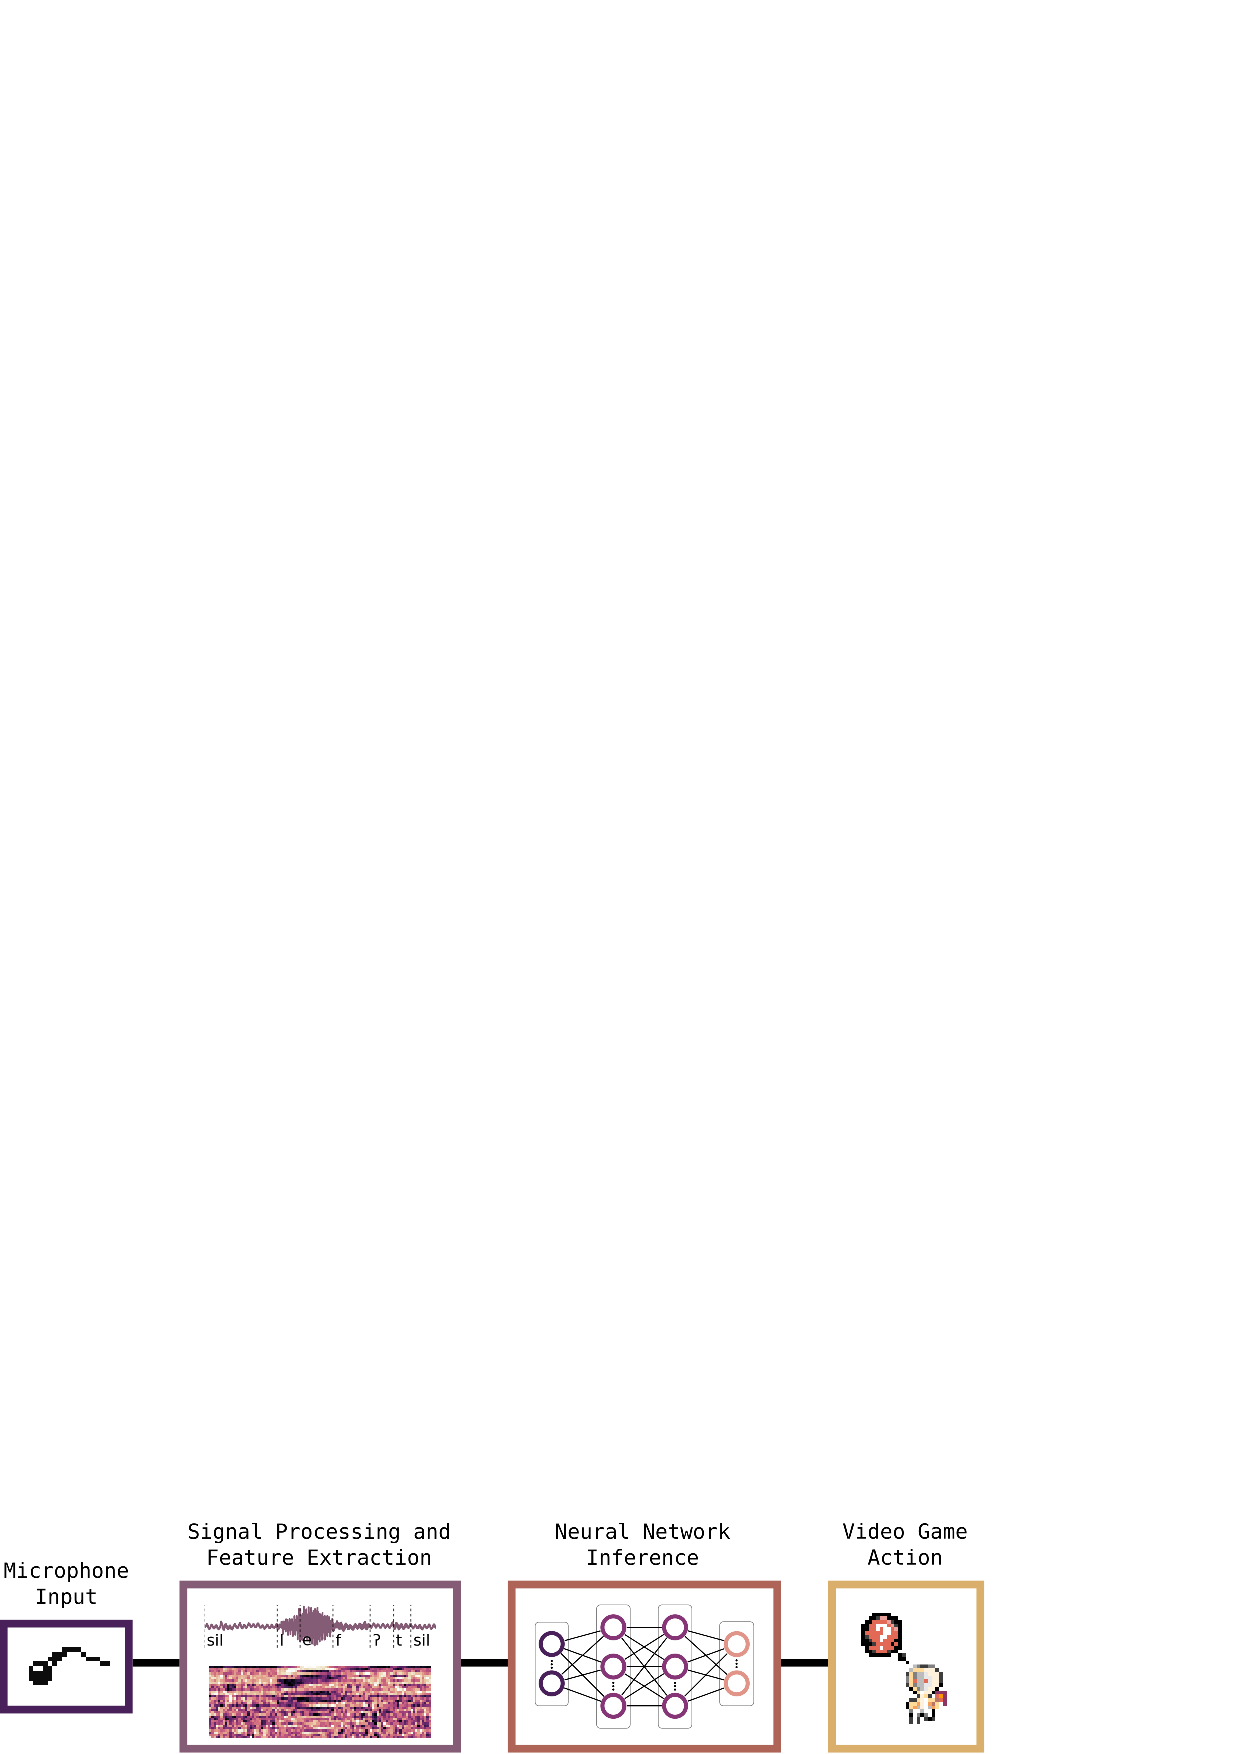
\includegraphics[width=0.95\textwidth]{./1_intro/figs/intro_kws.pdf}
  \caption{Simplified process of key word spotting for video games.}
  \label{fig:intro_kws}
\end{figure}
\FloatBarrier
\noindent
In the semantic perspective, the controlling of game objects, should be short, clear and best done with single command words, referred as speech commands.
Single words are easier to detect in comparison to long sentences, for instance, it is easier to recognize the word \enquote{left} than the sentence \enquote{missile target on position x, y}.
The classification of those speech commands can be done with a KWS system composed of a neural network.
KWS is restricted by a limited set of selected key words, referred as vocabulary or class dictionary.
In terms of video games, the set of key words might have members like \enquote{left} or \enquote{right}, for example, to move an element within the game to either left or right respectively.
The limited set of key words is crucial to restrict the complexity of the recognition task, since in practical applications it is not necessary to cover all words in a natural language.
Especially in video games, where the game environment is restricted by rules, technical limits and play-ability, KWS is suited perfectly as an alternative or augmented control system.
The size of the vocabulary and the selected words are two parameters that influence on one hand the choice of the neural network architecture, evaluated on energy efficiency and accuracy performance and on the other hand the game experience over the controls a player can choose from.
If the vocabulary of a KWS system would be too large, the chance of confusion between two different key words grows naturally.
In many KWS applications it is absolutely necessary to include labels for \emph{background noise}, \emph{silence} and \emph{unknown words} in the vocabulary. 
This is especially interesting in \emph{wake word} applications, where a single key word must be detected over the previously mentioned labels representing all other possible words that can be spoken.
Also in video games those additional labels are useful to prevent the player from eliciting unintended commands accidentally through, for instance, loud background noise.
Therefore, a KWS system has the demand of being very accurate and fast in its classification of key words.

Nowadays KWS systems are considered no science-fiction anymore, assisting consumers in everyday situations, such as rendering simple control tasks as the triggering of a photo release button on a \emph{smartphone} with a single speech command.
Application like this create more awareness of KWS, or generally speaking of speech recognition tasks, in human society.
Unfortunately some consumer applications with integrated speech recognition systems, leave a bitter aftertaste in data privacy issues and energy consumption through an externally and extensive computational processing pipeline over corporate servers \cite{Tang2018}.
It is therefore important to create incorporated KWS systems that respect private user data and provide an efficient implementation to save energy consumption.

Video games are a potential application for KWS, until now however, there exist very few of them taking advantage of this special feature.
Reasons for that might be found in the history of video games itself, where players find themselves in fast paced arcade games and speech recognition was simply too slow.
Additionally the complexity of KWS and lack of training data are often two valid arguments for not considering the deployment of a KWS system in a video game.

The following two sections in this introduction will briefly show the contributions of this thesis and give an overview of upcoming sections.
In summary, the focus of this thesis lies on KWS with neural networks trained through supervised learning on a speech command dataset \cite{Warden2018}.
The best suitable solutions for speech commands classification in video games are presented and evaluated with special interests in Convolutional Neural Networks (CNN), Generative Adversarial Neural Networks (GAN), and Wavenets.

% contributions
% --
% contributions

\section{Contributions}
The most of the effort is put into evaluating Convolutional Neural Network (CNN) models with low computational footprints, such as in \cite{Sainath2015}.
Besides low computational footprint, the depth of layers is hold to a minimum, so that it is still possible to get information about feature maps from the trained CNN networks.
The dataset used for the Key Word Spotting (KWS) task of those networks, was the speech command dataset \cite{Warden2018}.
The input features of the CNN models are the Mel Frequency Cepstral Coefficients (MFCC).
The amount of MFCC cepstral coefficients was evaluated with either 12 or 32 cepstral coefficients and showed that no accuracy improvements are achieved with 32 cepstral coefficients compared to 12.
The enhancement of MFCC to 39-feature vectors with 12 cepstral coefficients was also evaluated and showed only small improvements of accuracies, but not significant ones.
A frame-based normalization was performed on MFCCs to suite them better for visualization and use them for Generative Adversarial Networks (GAN) training.
Evaluation of the frame-based normalization was done in terms of accuracy, shift and noise invariance on conventional CNN models.
Frame-based normalization showed significant worse accuracies (about 5 to 10\%), it takes a bit longer for training, but improved in many experiments the noise invariance properties than without.
From those experiments the 12 cepstral coefficients with frame-based normalization were picked for further experiments.

Another large evaluation topic was that of GANs. 
With frame-based normalization the Generator (G) network was able to create convincing fakes to fool the Discriminator (D) network.
However it was found, when G and D are trained for too long, an equilibrium state where both generate random guesses or fakes might happen and the result is noise samples from G and a discrimination of D with slight changes around $0.5$.
Therefore a second loss term for G was added to create samples that have some similarity measure to the input data.
This helped to create better fakes and did not lead into noisy equilibrium states.

From the adversarial training of GAN networks, it was evaluated how their obtained weights through training can contribute in CNN models for KWS of speech commands.
Transfer learning was used to, transfer the obtained weights from either D or G to the equivalent CNN model.
With this approach it was possible to significantly increase the accuracy performance with about $3\%$ with using weights from G.
It showed that the obtained weights of G from an adversarial training can be very valuable.

A completely different approach for KWS was the evaluation of a Wavenet \cite{Oord2016} model for classification.
However with the hope that without feature extraction, a low computational model can be used, turned out to be extremely false.
Wavenets need a huge amount of operations by processing each sample from the audio files of the dataset.
Further the performances turned out to be very bad.
Nevertheless this model is evaluated and results are provided in hope for future research.

% overview
% --
% intro overview of thesis

\section{Overview of this thesis and notations}\label{sec:intro_overview}
\thesisStateReady
%This thesis is organized such, that each chapter leads to the next one and guiding someone who is interested in creating her own KWS game to follow through the process and challenges that might appear.
This thesis is organized that each chapter connects to the next one in a typical processing stage to create a KWS game.
% prev
After this introduction, \rsec{prev} provides information about previous and related work.
A small history sections about neural networks is given and important works on neural network architecture regarding this thesis are referrenced.
Further some works are presented that influenced and motivated this thesis.
Others works provide benchmarks on the used speech commands dataset or describe neural networks models that perform well on speech.
%In any way it is important to know, what is happening in the field of KWS and in which direction research is heading towards.
%Some works are used as motivation and some to get an idea.
% signal
\rsec{signal} is about audio signals processing and the extraction of meaningful features, such as MFCCs.
The feature extraction is explained in detail and examples are shown to visualize the results.
% neural networks
The used neural network architectures are described in \rsec{nn}. 
Further some theory of neural networks in general, CNNs, GANs and Wavenets is provided and highlighted with training results from experiments.
% experiments
In the \rsec{exp} information about the dataset and feature extraction is given and the experiments are presented.
Experiments are done on feature selection to determine the best suitable feature constellation the further experiments.
Adversarial pre-training is evaluated and Wavenets are compared to results from CNN based architectures.
% game
\rsec{game} describes the online and classification scheme in a possibile video game application.
Further some game design is presented and everything that is important for a KWS video game.
% conclusion
The thesis finishes with the conclusion in \rsec{conclusion}.


% visual guidance
%\subsection{Visual Guidance}\label{sec:intro_overview_visual}
%To get a better overview on the presentation of data and results, context specific color color-schemes are used within this thesis.
% There exist following context abstractions:

% \begin{itemize}
%     \item raw waveforms from soundfiles
%     \item extracted features, e.g. MFCCs
%     \item weights matrices of neural network models
%     \item training scores
% \end{itemize}

% ipa
\subsection{International Phonetic Alphabet}\label{sec:intro_overview_ipa}
The International Phonetic Alphabet (IPA) defines phonetics by human speaking sounds, where each symbol represents one specific sound.
A word formed with letters from a language alphabet, does not necessaryily represent the pronunciation of that word, therefore many dictionaries provide an IPA transcription so that no misconceptions may happen.
The plots, in some sections within this thesis, contain phonetic transcriptions with IPA characters, some of the more special ones are described in \rtab{intro_overview_ipa}.

% ipa table
\begin{table}[ht!]
\begin{center}
\caption{Some IPA and silence symbol with description.}
\begin{tabular}{ M{2cm}  M{9cm} }
\toprule
\textbf{IPA Symbol} & \textbf{Meaning} \\
\midrule
\textturnv & back vowel: \enquote{A}, open-mid roundend mouth \\
\textupsilon & back vowel: between \enquote{O} and \enquote{U}, nearly closed rounded mouth\\
\textinvglotstop & glottal stop\\
\midrule
sil & silence, no ipa symbol!\\
\bottomrule
\label{tab:intro_overview_ipa}
\end{tabular}
\end{center}
\end{table}
\FloatBarrier
\noindent



% math
\subsection{Mathematical Notations}\label{sec:intro_overview_math}
The mathematical equations or expressions are following some criteria.
Vectors and scalars are usually written in small letters with no special indication for vectors and matrices are written in capital letters.
The dimension of vectors and matrices are usually provided, such as $x\in\R^n$ or $X\in\C^{m \times n}$, or follow from the context.
Many letters like $n$ or $x$ are likewise used in different sections, but with different meaning and representations and should hopefully not confuse the reader of this thesis.
The letters $m$ and $n$ usually describes the length of a signal, $x$  and $y$ often represents input and output variables, etc.


% --
% background section

\chapter{Background}\label{sec:back}
This section provides fundamental background information regarding KWS, neural networks and video games.
The KWS task is described mathematically to express the actual speech recognition problem.
Notes on neural networks explain common properties and terms in their application.
Research questions are listed and give a deeper insight in common challenges of implementing a KWS system into a video game.

% disciplines
% --
% Intro of key word spotting

\section{The Key Word Spotting Task}\label{sec:intro_kws}
\thesisStateRevised
As described in \rsec{intro}, KWS is the task of classifying speech signals of spoken words to single key words out of a set of key words.
The set of key words $S$, also called vocabulary, can be defined as:
% kws dict
\begin{equation}\label{eq:intro_kws_dict}
	S \coloneqq \{s_i \mid i = 0, 1, \dots, L\}
\end{equation}
with a total number of $L$ key words denoted individually as $s_i$ for each key word.
The task is to select the key word closest to the spoken word from the user, denoted as target $t$.
The target does not necessarily have to be a member in the set of key words $S$, in fact it can be any arbitrary word.
With the abstract formulation:
% kws task
\begin{equation}\label{eq:intro_kws_task}
	\hat{s} = \underset{s_i \in S}{\arg \min} \, \mathcal{D}(t, s_i)
\end{equation}
the most probable key word $\hat{s}$ can be predicted, where $\mathcal{D}$ is some kind of distance measure between two words.
The formulation in \req{intro_kws_task} is merely semantic, but KWS in computer systems must cope with various transformations of raw input samples of audio data denoted as $\bm{x} \in \R^n$, with a total number of $n$ samples.
From the audio data an inference to output class probabilities $\bm{y} \in \R^L$ with a total number of $L$ class labels or key words, can be processed for instance with a neural network containing a softmax function at its last layer (transforming the output of the last layer to probability values).
With the softmax output from a neural network, the most probable key word can be picked by:
\begin{equation}\label{eq:intro_kws_class}
	\hat{s} = \{s_i \mid \underset{i = 0, 1, \dots, L}{\arg \max} \, y_i\}
\end{equation}
if the highest value of $y_i$ for all $i$ refers to the most probable index or indices of a spotted key word or key words in the vocabulary.

In comparison to full Automatic Speech Recognition (ASR), where whole sentences need to be identified, key word spotting operates merely on the word level.
Therefore KWS is a bit easier to deploy and less complex than ASR.
On the other hand KWS systems, that are used in practical applications, must run very energy efficiently on low energy devices, such as mobile phones, and give immediate and accurate responses to the users. 
A good elaboration on the requirements of KWS systems can be found in the motivation section of \cite{Warden2018}.
% --
% Intro to neural networks

\section{Neural Networks for Key Word Spotting}\label{sec:intro_nn}
\thesisStateReady
Neural networks enable computers to automatically learn from data to be able to solve tasks such as pattern recognition in images or audio.
The examples or samples from the input data can be paired with annotations, denoted as \emph{labels} or \emph{classes}.
If the label information of each example is used during the \emph{training} of a machine learning system, such as a neural network, it is called \emph{supervised learning} otherwise it is called \emph{unsupervised learning}, however supervised learning is more commonly applied.

%The big advantage of neural networks is that they are able to cope with huge amounts of input variables per data example and are able to extract their own features of those inputs through many layers within the network.
The big advantage of neural networks is that they are able to cope with large amounts of input variables per data example.
Considering a raw waveform file of merely \SI{1}{s} time duration, sampled with \SI{16}{\kilo\hertz} would give a input size of 16000 features.
This huge amount of input features is even difficult for neural networks to learn from and usually a feature extraction stage is placed in between to reduce the input dimension.
For instance the computation of MFCCs, using 12 out of 32 coefficients and a time duration of \SI{0.5}{s} with a time shift of \SI{10}{\milli\second}, reduces the input feature size dramatically to $12 \times 50 = 600$, which is still a high number of input features, but much more affordable and faster to train.

%In this thesis, the word \emph{feature} has several meanings, one is as name of extracted data and therefore be the same as input variables. 
%Another is, that a feature is simply some kind of compressed representation of a high dimensional data.
Neural networks are able to learn own feature representations, selection and interpretation, rather than using hand-crafted ones done by humans with expertise in the application.
Note that hand-crafting features of a complex recognition task, is in most cases not even possible or extremely cumbersome.
So researchers prefer neural networks because of their easy deployment scheme and state of the art performances.
Further it enables everyone who is capable of using neural network tools, to create solution to rather complex problems usually solved by experts in the field, given there is enough data and processing power available.
Therefore elaborate feature extraction stages become less important to the users.
This on the other side may lead into less understanding of the actual problem and more \enquote{try and error} approaches of different neural network architectures and training parameters.
The energy consumption required to train large neural network with many parameters on a huge training dataset, shall not be forgotten, especially in times of climatic change.
Reusing pre-trained weights from renowned network architectures is a good way to reduce energy consumption in finding an optimal classifier for a specific task.
The re-usability of pre-trained weights is often named as \emph{transfer learning}. 
A small summary on transfer learning can be found in \cite{TransferLearning}.
%This led to the thinking that everyone, who owns data and computational power, is the superior of solving complex problems such as image or audio classifications.
%However it is not always like this rather negative example, when using neural network approaches.

The potential of neural networks in research are vast.
The observation on how the learning from data is done and what recognition patterns are obtained after training, might allow researchers and experts to better understand the problem or gain a different viewpoint on it.
%However if neural networks are observed on how they are able to learn from data and what recognition patterns they have obtained after training, it might benefit researchers and experts to better understand the problem or gain a different viewpoint on it.
%It is extremely interesting to work with them and get knowlege about how and why they are able to produce such good results.
%This again feedbacks experts to gain more understanding or a different viewpoint on the topic.
Especially when using Convolutional Neural Networks (CNN), researchers are actually able to observe and visualize the learned filters and interpret the results.
A very interesting example of investigating learned CNN filters is shown by Zeiler el. al. \cite{Zeiler2013}.
Other interesting subjects in research are generative models, such as Generative Adversarial Networks (GAN) \cite{Goodfellow2014}, which are able to create convincing samples from the learned data distribution.

Neural network architectures for speech recognition are a little bit different from image recognition, mainly because of the sequential nature of time signals.
However if time signals are restricted in time, that means limited to a fixed number of samples, and frequency features are extracted over that time span, then speech signals can be represented in 2D space (frequency and time) and classified like images.
That suggests that CNNs are reasonable network architectures for speech as well.
Another interesting architecture for audio signals is the Wavenet \cite{Oord2016}, because of its ability to process raw audio data.
%and were originally intended for speech synthesis, but could also be used for recognition tasks.



% --
% video games with speech commands

\section{Video Games with Speech Input}\label{sec:intro_games}
\thesisStateReady
Video games with speech inputs are a rarely seen occurrence in the gaming industry, though it is a very interesting and immersive way to interact.
Technically the voice of the player of the video game, has to be recorded by a microphone, therefore one additional requirement of being able to play the video game is to own a microphone, which however does not need to be high-end.
The input stream of a microphone can be processed through an online or realtime system to extract the input data for the classification system.
The classification system, such as a neural network, infers the input data and therefore hopefully the intention of the player to a real action within the game.
The processing scheme is easy to define, but not that easy to implement compared to other more hardware based input channels, such as a click on a keyboard button.
Also speech input is very slow compared to hardware input, where players interact within tens of milliseconds (the input lag of gaming controllers should ideally be under \SI{50}{\milli\second}).
This is not possible with speech, the player has to physically form a waveform representing the action in the game.
Further the waveform captured from the online system has to be pre-processed, feature extracted and classified to the best estimation of all the available key words in the games vocabulary.
Concluding this, a good estimate to create and process a speech input should ideally be under one second, the less the better for the playing experience.

Another important question is how many key words or speech commands, should be used for the vocabulary.
A high number of key words will increase the chance of confusion and a small number of key words restrict the possible actions a player can choose from.
The possibility to create separate classifiers with different sets of smaller vocabularies of speech commands arises depending on which commands the player actually needs in the actual scenario within the video game. For instance if the player is in a dialogue with a Non Player Character (NPC) it makes sense to reduce the vocabulary to only \{\enquote{yes}, \enquote{no}\} if those are the only actions to choose from.

The use of labels for background noise, silence and unknown words depends on the game and how the classification process is activated.
If the assumption is made that a player chooses only from the key words in the dictionary, then the label of unknown words is not really necessary.
However the unknown label would be very interesting if key words are not that common to a player, such as words from a different language or fantasy words.
The unknown label will therefore motivate the player to correctly pronounce the word itself, which could be also used in language learning games.
The labels for background noise and silence are useful if the activation of the classification process is initiated by the energy value of the input stream of the microphone.
A stroke on the microphone or loud background sound can therefore elicit an unwanted command within the game, if those labels do not exist.

In any case there are much problems to consider when using KWS in video games and probably therefore hinders game developers to produce more content with it.

%Maybe those issues and the complexity of the task hinders game developers to produce more content with Key Word Spotting.
% A speech input for video games is a spoken waveform, recorded through a microphone, from any speaker intending to inflict a certain change while playing a Video Game. 
% Certainly this spoken waveform has to be processed, such as other inputs channels have to be (like keyboard buttons pressed), so that its meaning can be understood by the computer system behind the game. 
% Although this processing of a waveform is much more complicated and prone to errors, compared to a simple click on the keyboard or mouse. 
% That might be one of the reasons why Speech Inputs are very rare to be found in Video Games, still they exist.

% research questions
% --
% research questions

\section{Research Questions for this Thesis}\label{sec:intro_rq}
This section formulates relevant research questions regarding KWS in video games.
Those research questions can be split into 3 parts:
\begin{enumerate}[label={Q.\arabic*)}, leftmargin=1.4cm]
  \item Signal processing and feature extraction of speech signals.
  \item Neural network training and classification for KWS.
  \item Video games with KWS.
\end{enumerate}
Note that the terms \enquote{key word} and \enquote{speech command} are often named interchangeably because speech commands are used as key words in the KWS system.
Not all research questions can be answered within the scope of this thesis.
Nevertheless, those questions can be asked and some solution concepts discussed.


% --
% signal

\subsection{Signal Processing and Feature Extraction Research Questions}\label{sec:intro_rq_signal}
Acquiring meaningful features from speech signals is essential for neural networks to operate on. 
The features are extracted from raw audio samples of a microphone input stream in a specific time interval.
Those retrieved features are further input to a neural network for the classification of speech commands.
The following Questions arise here:
\begin{enumerate}[label={Q.1.\alph*)}, leftmargin=1.75cm]
  \item Which time interval should be captured to represent a speech command?\label{it:q1-a}
  \item Does the signal processing have to be invariant to background noise and especially to game sounds?\label{it:q1-b}
  \item What are meaningful features for speech recognition?\label{it:q1-c}
\end{enumerate}
\noindent
\textbf{Question \ref{it:q1-a}:} 
The time required to fully pronounce a speech command is not fixed and varies from speaker to speaker, depending also on the intended prolongation a speaker adds to the word.
In practical applications however, a fixed time interval for a single speech command is convenient.
By restricting the time duration of the key words, the speaker has to pronounce the words within this time span.
For example, if a speaker pronounces the word \enquote{left} and requires a time duration of \SI{1}{\second}, hardly all is captured if the time interval is restricted to merely \SI{500}{\milli\second}.
Whether this \SI{500}{\milli\second} is sufficient for a correct classification, is subject for evaluation.
In the application of a video game, the user should preferably speak the commands with a short time duration so that the game can respond fast.
Problems might occur if the speech commands are spoken repeatedly and very hasty such that the time interval of consecutive commands overlap each other.
Ideally the time interval to represent a speech command would be flexible but this more difficult to implement than a fixed time interval.

\textbf{Question \ref{it:q1-b}:}
Usually the presence of low background noise should not be a problem for neural networks trained on a large enough data set. 
The game sounds might present a more difficult problem, when turned up too loud without the use of headphones. 
Therefore, the microphone will not only capture the voice of a speaker but also a fair amount of game sounds. 
This problem seems to be theoretically solvable as the shape of the nuisance is known and the amount of game sound in the audio stream could be attenuated sufficiently.
In practice this might be hard to solve without critically disturbing the signal of interest.
A solution to this problem would probably take too much time and effort and is therefore not evaluated within this thesis. 
However, playing a video game without game sound is unsatisfying and it would be a great contribution to tackle this problem in future work.

\textbf{Question \ref{it:q1-c}:} 
The determination of meaningful features for speech signals is a classical problem in speech recognition.
The essential composition of a word may help to understand the problematic better.
A word is a sequential combination of either vowels, such as \enquote{a} and \enquote{e}, or consonants \enquote{k}, \enquote{l}, with a certain length. 
In linguistics, for instance, it is possible to distinguish vowels with frequency peaks in a spectrogram, where a spectrogram is the magnitude squared of the frequency response of small time chunks over the time duration of a signal.
However, due to many different factors in voice generation involved in speakers, such as age, gender, nationality and physiology of the vocal tract, there is a huge variance in the pronunciation of words from different persons, which increases the difficulty of the problem.
A very common approach is to use MFCCs as features for speech recognition tasks.
Why MFCCs present reasonable features for speech, is described in detail in \rsec{signal_mfcc}.


% --
% neural networks

\subsection{Neural Network Implementation Research Questions}\label{sec:intro_rq_nn}
Neural networks for video games should ideally be very efficient and provide accurate classifications of input features.
The vocabulary in a KWS task has to be specified for the individual game and chosen from all class labels available in the dataset.
Each key word of the vocabulary is presented by one output node of the neural network architecture.
Following Questions can be asked in general:
\begin{enumerate}[label={Q.2.\alph*)}, leftmargin=1.75cm]
  \item Is there an appropriate dataset suited for KWS video games and with sufficient diversity available?\label{it:q2-a}
  \item What happens if an input feature represents a spoken word, which is not in the vocabulary (unknown key word) and how should this exception be handled?\label{it:q2-b}
  \item What is the best neural network architecture regarding classification accuracy and energy efficiency?\label{it:q2-c}
  \begin{enumerate}[label=(\roman*)]
    \item Can adversarial networks improve generalization?
    \item Are Wavenets a solution to this task?
  \end{enumerate}
\end{enumerate}
\noindent
\textbf{Question \ref{it:q2-a}:} 
The availability of a dataset for KWS video games can be answered right away, as there exists a speech commands dataset \cite{Warden2018} with enough and diverse data.
The dataset consist of 35 labels and contains commands for movement and numbers.
Further, it includes randomly selected words like \enquote{marvin} or \enquote{bird} intended to represent \emph{unknown} words for the KWS system.
It has to be noted that not every game idea can be realized with a restricted vocabulary.
Nevertheless, with commands for movement like \enquote{left} or \enquote{go} it is possible to move objects within a game and this can already be used for many game mechanics.
An aspect regarding efficiency, is to restrict the amount of key words in the vocabulary as much as possible such that a cheaper neural network architecture can be deployed, which of course should still be sufficiently good in its classification accuracy.

\textbf{Question \ref{it:q2-b}:} 
Without doubt, players will try out words that are not in the vocabulary (denoted as \emph{unknown} key words) and observe the response of the video game.
The ideal response would be to shown an indication to the player that the word is not present in the vocabulary. 
Nevertheless, it might happen that the similarity of an unknown key word is too close to a key word and an unintended action is triggered in the game. 
At the same time the neural network should not classify key words as unknown key words to ensure a satisfying game experience.
It is better to rely on that players are using key words for most of the time so that they are preferred over unknown key words.

\textbf{Question \ref{it:q2-c}:}
In the ideal case, video games with KWS do not slow down during the inference process of unknown input data.
The restriction of the amount of computations and time for the classification of key words is given by the minimum Frames Per Second (FPS) a video game is perceived as fluent.
That requires the FPS to not fall under a certain limit (usually 30 FPS in video games), otherwise the fluidity of the game is not guaranteed.
Therefore, several different neural network approaches with a low computational footprint have to be tested and compared against each other regarding classification rate and energy efficiency.
The transfer of weights from GANs is an interesting approach to evaluate whether the trained parameters are also useful for pure classification tasks in CNNs.
Wavenets have the advantage that they do not need a feature extraction stage but it is questionable whether the network design achieves a reasonable computational footprint.


% --
% video games

\subsection{Video Games with KWS Research Questions}\label{sec:intro_rq_games}
Video games that use KWS can create an unique playing experience but have to face certain challenges.
Following questions can be stated:
\begin{enumerate}[label={Q.3.\alph*)}, leftmargin=1.75cm]
  \item How should the onset of a key word be detected, so to reduce computations?\label{it:q3-a}
  \item What is the added value of KWS in the gaming experience of players?\label{it:q3-b}
  \item What do game developers have to consider, when designing a game with KWS?\label{it:q3-c}
\end{enumerate}
\noindent
\textbf{Question \ref{it:q3-a}:} 
It is crucial to reduce computations in a video game in order to keep it running fluently during high performance peaks.
Also the unnecessary processing of meaningless input data should be avoided as much as possible.
Ideally the key word classification is activated, when there is actually a speech command present, which however is not always trivial.
One possibility to indicate the onset of a key word is to perform the relatively efficient calculation of an energy value within a certain time interval of the raw input data stream and have a simple threshold value decide, whether a speech command is available. 
To avoid the consecutive triggering of onsets at each energy measure, the microphone and amplifier noise floor and the background sound (including the game sound) have to be less energy intensive than the speech signal obtained from the player.
Another approach similar to the push and talk principle, would be to indicate the onset of a key word with the click of a certain button on the keyboard.
The player is therefore able to control the exact onset of a key word and its length but requires an additional hardware based input channel.

\textbf{Question \ref{it:q3-b}:}
In certain video game scenarios, speech commands can be useful, interesting and enhancing for the gaming experience, in others they might even disturb the game play or even spoil it completely.
It cannot be generally stated whether it is worth to deploy a KWS system into a game, this depends on the game it is intended for.
As already noted in \rsec{intro_games}, KWS might be a great augmented control system for special kind of games to increase the immersion experience, especially for VR applications.
Also language learning games are an interesting application but usually require a huge vocabulary and therefore a phoneme based ASR system would be the better choice.

\textbf{Question \ref{it:q3-c}:}
Apart from the technical requirements involved in KWS systems, also the general game design with KWS has to be considered.
It certainly can be stated that KWS systems are not always reliable and therefore a main game mechanic solely based on it is not always preferred.
Furthermore, the time lag required to process speech commands to actual actions within the game should not be ignored.
The player should get on the one hand immediate and accurate feedback from the game and on the other hand be challenged while playing.
Further, by achieving both criteria it ensures that the game experience does not suffer from getting frustrating or tiresome.
Additionally it must be considered, that players might get exhausted by using speech commands consecutively in short intervals during the game.
Therefore, the players might prefer a game design where they have to use KWS only in special situations.
As general conclusion, it can be stated that a game developer has to design a KWS game with great care.
% --
% previous and related work

\chapter{Previous and Related Work}\label{sec:prev}
This chapter presents important works that had influenced this thesis.
The works can be separated in audio features, neural networks, key word spotting and video games with key word spotting.

% features
% --
% prev features

\section{Audio features}
The extraction of audio features from acoustic waveforms is important for data compression.
One of the most popular features are the Mel Frequency Cepstral Coefficients (MFCC), developed by
\cite{Mermelstein1980} in 1980.
They are motivated by the physiological human hearing system.

% neural networks
% --
% prev neural networks basics

\section{Neural Networks Basics Architectures}\label{sec:prev_nn}
\thesisStateNotReady
This section is a summary and history review of some specific neural network architectures used within this thesis.
The purpose is merely to give a slight overview of these architectures and the researchers that contributed to them.

% --
% prev history

\subsection{Historical Remarks on Neural Networks}\label{sec:prev_nn_history}
The first step towards computational neural networks, as we know them today, was the introduction of the so called \enquote{Perceptron} by Rosenblatt in the year 1958 \cite{Rosenblatt1958}. 
The idea of the Perceptron emerged from physiologists, trying to model a physiological neural network in computational terms. 
This first model was based on the information processing of the retina (input nodes), which passes through several physiological neural networks (hidden nodes) and finally elicit an action or decision (output nodes).
Publishing his work and implementing those ideas in an actual computer system (at those time computers were huge boxes), Rosenblatt kicked of the domain of computational learning systems.
The race of finding best neural network architectures for specific regression or classification tasks had begun.

Another big advance in the history of neural networks, was the introduction of a very famous learning algorithm known as \enquote{Backpropagation}, evolved by several authors at the same time \cite{LeCun1986} and \cite{Rumelhart1986} in the late 80s. 
Even nowadays, 35 years after introducing backpropagation, it is still the \emph{de facto} standard in training neural networks.
Nowadays backpropagation is implemented in every machine learning framework for neural networks as its core element.
Such frameworks are for instance \texttt{Pytorch} or \texttt{Tensorflow} and of course many others, handling the gradient calculation and backpropagation algorithm of those gradients in the background.

The neural networks reputation during the time until now, was not always seen that splendid.
The general problem of handling overfitting (prevent networks from learning data samples by heart) and generalize better on unseen data, is still an open issue in many applications.
Some mathematicians working in the field of statistical methods in learning theory for pattern recognition, regard neural networks as being not meaningful in the advance of learning theory, such as one quote from \cite{Vapnik1995} of Vapnik's book in 1995 about natural learning theory:

\begin{quote}
...In spite of important achievements in some specific applications using neural networks, the theoretical results obtained did not contribute much to general learning theory...
\end{quote}

This quote is a bit tough, but unfortunately true in some sense. 
The complexity of neural networks with many layers, makes the tracing of the learning process very difficult.
No concrete formulas, apart from the calculation of gradients, can exactly explain what neural networks are actually learning.

Therefore on one side there were the classical statistical learning methods, the most famous one called Support Vector Machines (SVM) \cite{Cortes1995} and one the other side there were neural network approaches.
Over a long period of time SVMs were preferred over neural networks, because they were better understood with profound mathematical methods and achieved state of the art performance with sophisticated feature extraction algorithms.
Not until 2012, neural networks gained more popularity again by scoring new benchmarks in image classification tasks with one famous paper \cite{Krizhevsky2012}, by beating the previous benchmark with a significant score.
Deep Learning was the new key to success, with network architecture consisting of many layers and a large amount of parameters to train.
Also in audio and language processing tasks, such as Automatic Speech Recognition (ASR) and Natural Language Processing (NLP), the famous Hidden Markov Models (HMM) and other statistical methods get more and more replaced by neural networks.

With this remarks the short review on neural network history are closed and readers may forgive that not more details are presented and more papers referenced.
The interested reader is recommended to look through the references of the above mentioned papers for finding more detailed informations about its interesting history.


% --
% convolutional nets

\subsection{Convolutional Neural Networks}\label{sec:prev_nn_cnn}
Convolutional Neural Networks (CNNs) are a special class of neural networks, that are able to incorporate spatial information from the input data, with the application of convolutional filtering to create feature maps.
Spatial information is very important in images, where neighboring pixels are related to each other.
The same holds for audio, but in only one dimension and with a higher amount of samples.
Convolutional filters are very commonly applied in image processing tasks, such as denoising or other enhancements of images.
In audio processing, a classical application of convolutional filters is a simple average filter of the signals energy, to determine onsets like the start of a speech signal.

Still it took relatively long till convolutional filters were a common and a widely used asset in neural network architectures.
The general concepts of CNNs with feature maps (outputs of applied convolutional filters) and weight sharing through convolutional filters, were examined by LeCun et. al. on handwritten postal codes in 1989 \cite{LeCun1989_Generalization}.
Further research and experiments on the famous MNIST dataset of handwritten digits, were done in the late 90s \cite{LeCun1998} and asserted the success of CNNs.
A classical convolutional layer in CNNs usually consists of multiple convolutional filters with trainable weights and an additive bias terms per filter, followed by a non-linear activation function.
More details about CNNs is presented in
%Since then many famous image recognition models were introduced that incorporated CNNs and achieved state of the art performances.

%This is one reason why CNNs are so practicable for image recognition tasks and usually state of the art image recognition architectures have some kind of convolutional neural network implemented within.

%With their restricted and highly spatial connections and weight sharing through convolutional filters, they are an valuable asset no researchers should miss when working with images or audio recognition.

  
% best quote ever
%It is trivial to design a machine that learns very quickly, does not generalize, and requires an enormous amount of hardware. 
%In fact this learning machine has already been built and is called a Random Access Memory.


% --
% recurrent neural networks

\subsection{Recurrent Neural Networks}\label{sec:prev_nn_rnn}
Recurrent Neural Networks (RNN) are a type of neural networks, that are using feedback loops from the output of each node back to its input.
With those feedback loops it is possible to input sequential data with no fixed length restrictions.
%The information state is stored within the network.
RNNs are known to be hard to train because of the well known exploding or vanishing gradients problem.
This problem can be solved by using so called Long Short Time Memory (LSTM) that are incorporating gates for the information storage in each cell. 
However the LSTM cell also increases the amount of parameters to be trained for each node and backpropagation over a large amount of time steps is computationally intensive.

Through their design to capture sequential data, RNNs are commonly used in speech recognition tasks.
However they are not subject in this thesis, the interested reader if referred to a good comprehension in \cite{Staudenmeyer2019} with further references upon RNN works.


% --
% wavenets

\subsection{Wavenets}\label{sec:prev_nn_wavenet}
Processing raw audio data as inputs to neural networks seemed to be difficult for a long time.
This is mainly due to their huge amount of input data. 
Consider a \SI{1}{\second} audio file with a sampling rate of \SI{16}{\kilo\hertz} give 16000 samples and therefore a 16000 dimensional input vector.
Recently neural network architectures emerged with the ability to process raw audio samples.
One very prominent architecture, originally intended for natural speech generation, is the so called \emph{Wavenets} \cite{Oord2016}.

With the \emph{dilated convolution} and a quantization of the audio sample values, Wavenets can afford to process this huge amount of inputs.
Wavenets are in some sense similar to RNNs, because they also use outputs from previous time steps, but the implementation of wavenets is much more efficient, such as the quote from \cite{Oord2016} states:
\begin{quote}
  %Recurrent neural networks such as LSTM-RNNs (Hochreiter & Schmidhuber, 1997) have been a key component in these new speech classification pipelines, because they allow for building models with long range contexts. 
  ...With WaveNets we have shown that layers of dilated convolutions allow the receptive field to grow longer in a much cheaper way than using LSTM units...
\end{quote}


% --
% adversarial nets

\subsection{Generative Adversarial Neural Networks}\label{sec:prev_nn_adv}
Generative Adversarial Neural Networks (GAN) are motivated by Game Theory, in a way that they contain usually two separate networks, denoted as players, playing a game against each other.
The game hereby is to outperform the other player in an adversary task.
The idea of GANs emerged from Goodfellow in 2014 \cite{Goodfellow2014}, where one player (network) produces fake images, that are similar to real ones and the other player has to detect if it given image is a real or fake one.
Both players are therefore improving themselves upon each other, to either create more realistic fakes or to detect fakes from reals with low error rates.

In this thesis, the concept of GANs is used for pre-training weights to hopefully improve generalization and performance in a CNN network.
% --
% prev history

\subsection{Historical Remarks on Neural Networks}\label{sec:prev_nn_history}
The first step towards computational neural networks, as we know them today, was the introduction of the so called \enquote{Perceptron} by Rosenblatt in the year 1958 \cite{Rosenblatt1958}. 
The idea of the Perceptron emerged from physiologists, trying to model a physiological neural network in computational terms. 
This first model was based on the information processing of the retina (input nodes), which passes through several physiological neural networks (hidden nodes) and finally elicit an action or decision (output nodes).
Publishing his work and implementing those ideas in an actual computer system (at those time computers were huge boxes), Rosenblatt kicked of the domain of computational learning systems.
The race of finding best neural network architectures for specific regression or classification tasks had begun.

Another big advance in the history of neural networks, was the introduction of a very famous learning algorithm known as \enquote{Backpropagation}, evolved by several authors at the same time \cite{LeCun1986} and \cite{Rumelhart1986} in the late 80s. 
Even nowadays, 35 years after introducing backpropagation, it is still the \emph{de facto} standard in training neural networks.
Nowadays backpropagation is implemented in every machine learning framework for neural networks as its core element.
Such frameworks are for instance \texttt{Pytorch} or \texttt{Tensorflow} and of course many others, handling the gradient calculation and backpropagation algorithm of those gradients in the background.

The neural networks reputation during the time until now, was not always seen that splendid.
The general problem of handling overfitting (prevent networks from learning data samples by heart) and generalize better on unseen data, is still an open issue in many applications.
Some mathematicians working in the field of statistical methods in learning theory for pattern recognition, regard neural networks as being not meaningful in the advance of learning theory, such as one quote from \cite{Vapnik1995} of Vapnik's book in 1995 about natural learning theory:

\begin{quote}
...In spite of important achievements in some specific applications using neural networks, the theoretical results obtained did not contribute much to general learning theory...
\end{quote}

This quote is though, but unfortunately it is true in some sense. 
The complexity of neural networks make them not tractable in their learning process.
No concrete formulas, apart from the calculation of gradients, can exactly explain what neural networks are actually learning.

Therefore on one side there were the classical statistical learning methods, the most famous one called Support Vector Machines (SVM) \cite{Cortes1995} and one the other side there were neural network approaches.
Over a long period of time SVMs were preferred over neural networks, because they were better understood in their mechanism and achieved state of the art performance with sophisticated feature extractions algorithms at that time.
Not until 2012 neural networks gained more popularity again, scoring new benchmarks in image classification tasks with one famous paper \cite{Krizhevsky2012}.
Deep Learning was the new key to success, with network architecture consisting of many layers and a large amount of parameters to train.

Here this short review on history shall be stopped and readers may forgive that not more details are presented and more papers referenced.
The interested reader is recommended to look through the references of the above mentioned papers for finding more detailed informations.

% --
% prev convolutional nets

\subsection{Convolutional Neural Networks}\label{sec:prev_nn_cnn}
Convolutional Neural Networks (CNNs) are a class of neural networks, that are able to incorporate spatial information with the application of convolutional filtering.
Spatial information is very important in images, where neighboring pixels are releated to each other.
The same holds for audio, but in only one dimension and with a higher amount of samples.
Convolutional filters are very commonly applied in image processing tasks, such as denoising or other enhancement of images.
In audio processing, a classical application of convolutional filters is a simple average filter of the signals energy, to determine onsets like the start of a speech signal.

Still it took relatively long till convolutional filters were a common used asset in neural network architectures.
The general concepts of CNNs with feature maps (convolutional filters) and weight sharing through those feature maps
were examined by LeCun et. al. on handwritten postal codes in 1989 \cite{LeCun1989_Generalization}.
CNNs were introduced and examined by LeCun et. al. on handwritten digits of the MNIST dataset in the late 90s
\cite{LeCun1998}.
%Since then many famous image recognition models were introduced that incorporated CNNs and achieved state of the art performances.

%This is one reason why CNNs are so practicable for image recognition tasks and usually state of the art image recognition architectures have some kind of convolutional neural network implemented within.

%With their restricted and highly spatial connections and weight sharing through convolutional filters, they are an valuable asset no researchers should miss when working with images or audio recognition.

  
% best quote ever
%It is trivial to design a machine that learns very quickly, does not generalize, and requires an enormous amount of hardware. 
%In fact this learning machine has already been built and is called a Random Access Memory.

% --
% prev recurrent neural networks

\subsection{Recurrent Neural Networks}\label{sec:prev_nn_rnn}
Recurrent Neural Networks (RNN) are a type of neural networks, that use a feedback loop of their output over time.
It is therefore possible to store relevant input information over a fixed time span.
The neural network architecture can then be seen as unrolled over time.
However this unrolling multiplies the per time instance network architecture for each additional time instance,
which easily becomes a huge network.
Also RNNs are known to be hard to train because of exploding or vanishing gradients.
This problem can be solve with using so called Long Short Time Memory (LSTM) neural networks incorporating gates for the information storage in each cell. However the LSTM cell also increases the amount of parameters to be trained.
Through their design to capture sequential data, Recurrent Neural Networks are commonly used in speech recognition tasks.
However they are not regarded in this thesis because of being to cost intensive for a video game deployment.
The interested reader might read a good comprehension in \cite{Staudenmeyer2019}.


% --
% prev adversarial nets

\subsection{Adversarial Neural Networks}\label{sec:prev_nn_adv}
Adversarial Neural Networks are motivated by Game Theory, in a way that they incorporate usually two separate networks, denoted as players, playing a game against each other.
The game hereby is to outperform the other player in a specific task.
The idea of creating generative networks emerged from Goodfellow in 2014 \cite{Goodfellow2014}, where one player (network) produces fake images, that are similar to real ones and the other player has to detect if it given image is a real or fake one.
Both players are therefore improving themselves upon each other, to either create more realistic fakes or to detect fakes from reals with low error rates.

% --
% prev wavenet

\subsection{Wavenets}\label{sec:prev_nn_wavenet}

Processing raw audio data as inputs to neural networks seemed to be difficult for a long time.
This is mainly due to their huge amount of input data, consider a \SI{1}{\second} audio file with a sampling rate of \SI{16}{\kilo\hertz} yield into 16000 samples and therefore a 16000 dimensional input vector.
Recently neural network architectures emerged with the ability to process raw audio samples.
One very prominent architecture, originally intended for natural speech generation, are so called \emph{Wavenets} \cite{Oord2016}.

With a smart convolution technique called \emph{dilated convolution} and a quantization of the audio sample values, wavenets could afford to process this huge amount of raw audio inputs.
Wavenets are in some sense similar to RNNs, because they also use outputs from previous time steps, but the implementation of wavenets is much more efficient, such as the quote from \cite{Oord2016} states:
\begin{quote}
  %Recurrent neural networks such as LSTM-RNNs (Hochreiter & Schmidhuber, 1997) have been a key component in these new speech classification pipelines, because they allow for building models with long range contexts. 
  ...With WaveNets we have shown that layers of dilated convolutions allow the receptive field to grow longer in a much cheaper way than using LSTM units...
\end{quote}

% KWS for speech commands
% --
% prev key word spotting

\section{Key Word Spotting with Neural Networks}\label{sec:prev_kws}
\thesisStateNotReady
Some important works regarding KWS with neural networks are presented here. 
The aspect of energy efficients is very important within this thesis, because of the deployment of a KWS system in a video game.
Further the neural network architectures evaluated in this thesis are trained and tested on an already profoundly examined speech command dataset \cite{Warden2018} with many different solution concepts operating with neural networks. 
A benchmark is therefore given on classification accuracies on the test set of this dataset.


% --
% energy efficient

\subsection{Energy efficient solutions}
In video games the processing and classification of speech commands has to run in real-time and therefore a low computational footprint is needed for the neural networks.
One of the most famous papers on low computational footprint regarding KWS systems is from Sainath et. al. in 2015 \cite{Sainath2015}.
Two neural networks architectures are chosen from this paper, one is a traditional CNN network for comparison and the other is a limited multipliers network with a CNN striding only in the frequency axis.
Both networks are described in detail in \rsec{nn_arch}.

A deployment of a KWS system on microcontrollers is examined in \cite{Zhang2017}. 
Different neural network architectures were evaluated regarding their memory usage and operations per inference.


% --
% benchmark

\subsection{Benchmark Networks for this thesis}\label{sec:prev_kws_benchmark}
First it is to mention that the speech command dataset \cite{Warden2018} consists of raw audio data in the \texttt{.wav} format and there is no pre-processing or feature extraction done beforehand.
Also it is up to the users for which labels are to be selected.
The main idea however is to choose the \emph{core words} as classification labels and add an unkown label for the \emph{auxiliary words} words.
Also a separate noise or silence label can be added from given noise data files.
More details are presented in \rsec{exp_dataset}.

Therefore it is difficult to compare scores between two different papers.
Still the classification task is not an easy one in any constellation of chosen labels or feature extraction and usually everything that has a accuracy score over 85\% for at least 7 - 10 labels is already pretty good.
A good overview of actual benchmark scores regarding the speech command dataset is given in \cite{PaperswithcodeKWS}.





% games
% --
% prev games

\section{Video Games with Key Word Spotting}\label{sec:prev_kws_games}
Very few papers are tackling KWS specifically tied to video games and most research is conducted on gaining the best accuracies on datasets and setting new benchmark scores on them.
Nevertheless a research paper found, was that of a multiplayer video game intended for children presented in \cite{Harshavardhan2015}, which evaluates challenges when children are playing video games, such as repetitive and overlapping commanding.
On the other hand there are plenty of real world applications for KWS and ASR using available toolkits.
One very powerful tool for speech commanding widely used for video games is \texttt{VoiceAttack} running on \enquote{Windows Speech Recognition} \cite{Xiong2017}.
With \texttt{VoiceAttack} it is possible to specify own voice commands that are triggering combinations of keyboard clicks and therefore can be used to elicit actions in video games.
The applications are vast and flexible and can be applied in any game by running the program in the background.
An actual video game with integrated speech commanding ability, running with the \texttt{PocketSphinx} \cite{Huggins2006} speech recognition system, is \texttt{In Verbis Virtus}, where the players are able to cast spells by speaking out fantasy words after clicking an activation button as onset indication.
% --
% theory

\chapter{Theory}
This chapter contains the theoretical foundations of developing a Key Word Spotting system with Neural Networks for Video Games. 
In particular the signal processing and feature extraction is explained and visualized with many examples.
The same holds fo the machine learning part were central concepts of applied methods are discussed and shown.
At last it is important and has to be considered when building a video game with speech command inputs.

% sp
\input{./3_theory/theo_signal.tex}
\input{./3_theory/theo_signal_raw.tex}
\input{./3_theory/theo_signal_spectogram.tex}
\input{./3_theory/theo_signal_mfcc}

% ml
\input{./3_theory/theo_ml.tex}
\input{./3_theory/theo_ml_nn_arch.tex}
\subsection{Adversarial Training Theory}\label{sec:adv_theory}
Working with adversarial Neural Networks is quite interesting, as two separate Networks are challenge themselves against each other to improve their performance.
The paper from Goodfellow et. al. \cite{goodfellow2014} describes a game between two Neural Networks (players), where one player has the role of creating fakes and the other must determine if it is real or fake.
The Network who creates fakes is called Generator (G) and the other Network who has to decide about fake or not is called Discriminator (D).
The Generators goal is to create fakes that look like reals, so that D makes mistakes and classifies a fake as a real.
On the other hand the Discriminator is constantly improving itself as well, so that fakes from G can be detected.

This approach works remarkably well as generative network, producing fakes that are astonishing similar to real ones.
In the mentioned paper, this was applied to images and not for audio.
But if the audio waveform is presented as spectogram or mfcc with fixed frame size, it is the same as an image,
where one dimension is time and the other frequency.

So far a generative network does only produce fake images and a discriminative network can only output a one dimensional (probability) output, to decide if it is fake or not.

The idea now is not to use either of these networks, but to use transfer learning in the sense to reuse the convolutional layers both networks achieved during their game, in another network with classification purpose on multiple labels.

\subsubsection{Questions that arise}
There are several questions that arise regarding Adversarial Training:
\begin{enumerate}[label={Q.\textgoth{A}.\arabic*)}, leftmargin=1.4cm]
  \item Do the Network Architectures of G and D have to be the same but transposed?
  \item Does the value space of in and outputs, for D and G respectively, have to be limited e.g. [0, 1] done by e.g. frame normalization, or sigmoid output?
  \item What loss function works well for training?
  \item How long should be trained?
  \item When transfering weights to another network, should the weights from G or D be transfered?
  \item Whats the benefit of all this?
\end{enumerate}

To illustrate the idea an example is shown of the labels L5 (left, right, up, down, go).

The adversarial trained conv layer weights of the individual labels, can be stacked together an used to initialize another network.
An example of this method is shown in \rfig{ml_adv_example}, where the initialzation pattern changes to get more structures and further patterns to be good at classification. However the Basic Pattern from the adversarial training stays the same, which is a good sign, so that the network is able to use this trained weights.

\begin{figure}[!ht]
  \centering
    \subfigure[c1 trained]{\includegraphics[width=0.45\textwidth]{./3_theory/figs/ml_adv_example_c0}}
    \subfigure[c1 init]{\includegraphics[width=0.45\textwidth]{./3_theory/figs/ml_adv_example_c0_init}}
    \subfigure[c2 trained]{\includegraphics[height=0.45\textwidth]{./3_theory/figs/ml_adv_example_c1}}
    \quad
    \subfigure[c2 init]{\includegraphics[height=0.45\textwidth]{./3_theory/figs/ml_adv_example_c1_init}}
  \caption{Adversarial Training Example: Convolutional layers pretrained with adversarial training on each label separately.}
  \label{fig:ml_adv_example}
\end{figure}
\FloatBarrier
\noindent

For this example in adversarial training, 8 feature maps of the first layer were used for each label, also they belong to the Generator Network G or decoder (dec). In Convolutional Networks, each previous layers feature map creates a new set of feature maps in the next layer.
An example of this label training is shown in \rfig{ml_adv_example_label} with feature maps [(1, 8), (8, 8)] of the convolutional layers

\begin{figure}[!ht]
  \centering
    \subfigure[left c1 enc]{\includegraphics[width=0.45\textwidth]{./3_theory/figs/ml_adv_example_label_left_c0_enc}}
    \subfigure[left c1 dec]{\includegraphics[width=0.45\textwidth]{./3_theory/figs/ml_adv_example_label_left_c0_dec}}
    \subfigure[left c2 enc]{\includegraphics[width=0.45\textwidth]{./3_theory/figs/ml_adv_example_label_left_c1_enc}}
    \subfigure[left c2 dec]{\includegraphics[width=0.45\textwidth]{./3_theory/figs/ml_adv_example_label_left_c1_dec}}
  \caption{Adversarial Training example of label training with label \enquote{left}.}
  \label{fig:ml_adv_example_label}
\end{figure}
\FloatBarrier
\noindent

Those label trained weights can then simply be stacked into the new parameters of a classification network, but it is important that the layers are stacked not randomly, so that the trained connections are still correct.








% game
\input{./3_theory/theo_game.tex}
\chapter{Practice}
The practical part of this thesis can be found in this chapter.
It gives information about the Datasets and feature extraction of its data used for training the Neural Network architectures.
The dataset details and properties of the sound files are presented.
Some sound examples and their feature representation of the datasets are shown and the quality and diversity of recorded samples is mentioned.

Also this chapter includes the evaluation of the Neural Network models and the evolution process of the individual approaches used for speech command classification.
Also the implementation of the Key Word Spotting system and some Game Design ideas of possible applications with speech commands are given.


% dataset
\input{./4_practice/prac_dataset.tex}
% --
% Speech Commands dataset

\subsection{Speech Commands Dataset}
The Speech Command Dataset \cite{warden2018} is a very diverse dataset consisting of over thousands of different speakers. This dataset is by any means no clean dataset recorded by professionals, if anything it is the opposite. 
The audio files are not normalized, there are samples with inconsistent sample numbers and some examples are prone with too much noise or even noise only.
And its still great, because there is no need for a perfect dataset and one can be happy that there exists one with this amount of diversity and free of access.
In fact maybe its even better to have an unclean dataset, so that invariances against noise are learnt and do not have be added by hand.

\begin{figure}[!ht]
  \centering
    \includegraphics[width=0.65\textwidth]{./4_practice/figs/a_dataset/wav_grid_c30}
  \caption{Random samples from the Speech Command Dataset, one per class. Pre-processed and normalized raw audio data.}
  \label{fig:wav_grid_c30}
\end{figure}
\FloatBarrier
\noindent

\subsubsection{Extraction for Training}
The Speech Commands Dataset is extracted before it is used for training. 
To reduce computations in the evaluation process of Neural Networks, it was important to reduce the number of classes and examples per class to an suitable number.
In the Evaluation of Neural Networks the datasets the references in \rtab{dataset_refs} are used

\input{./4_practice/tables/tab_dataset_refs.tex}
% --
% my dataset

\subsection{My own Dataset}
The author of this thesis recorded some speech command samples by himself and used it as own test set in evaluating trained models in the machine learning part. No self recorded files are used within the training set, so that it can be shown that unseen voice characteristics are classified correctly.
All examples of my own dataset are illustrated in \rfig{dataset_wav_grid_my} in raw audio format.

\begin{figure}[!ht]
  \centering
    \includegraphics[width=0.65\textwidth]{./4_practice/figs/dataset_wav_grid_my}
  \caption{My wav grid}
  \label{fig:dataset_wav_grid_my}
\end{figure}
\FloatBarrier
\noindent

% machine learning
\section{Machine Learning Evaluation}\label{sec:ml}
In this section, the machine learning evaluation of the mentioned Neural Network Architectures, denoted here also simply as models, are presented.
The training details are listed to give the reader an overview of the selected parameters for training, it should also give a shorten reference, so that not all parameters must be listed in the plots. 
The training and evaluation consists of following evaluation tasks:
\begin{enumerate}
  \item Feature Selection
  \item Adversarial Training
\end{enumerate}

% --
% ml details

\subsection{Training Details}
We can separate the training details into following parameters to select from:
\begin{enumerate}
  \item Dataset parameters
  \item Features extraction parameters
  \item Feature selection
  \item Transfer Learning parameters
  \item Machine Learning parameters
\end{enumerate}
The dataset parameters are the information of what labels from the dataset are used and how many examples per labels, shown in \rtab{dataset_refs}.
The feature extraction parameters simply give information about how features are extracted, e.g. this includes the hop size, frame size, filter bands of the MFCC, etc.
The feature selection is the information about what input feature groups are used in the training, e.g. use cepstral coefficients only, or add delta and energy features, their references are shown in \rtab{dataset_feature_groups}.
The Transfer Learning parameters are pre-trained weights for the actual neural network architecture to be trained.
This could be only the first convolutional layers or entire networks but here all convolutional layers from an adversarial training are considered. 
The Abbreviations for training parameters can be specified as listed in \rtab{tab_ml_details_adv}
\input{./4_practice/tables/tab_ml_details_adv.tex}

The Machine Learning parameters are classically training parameters such as learning rate, number of epochs, etc.
Their selection and references are listed in \rtab{tab_ml_details_train_params}

\begin{table}[ht!]
\begin{center}
\caption{All training parameters used within this thesis and their abbreviations.}
\begin{tabular}{ M{2cm}  M{5cm} }
\toprule
%\multicolumn{4}{c}{\textbf{Feature Groups}} & \multicolumn{2}{c}{\textbf{Accuracy}} \\
\textbf{Abbreviations} & \textbf{Meaning}\\
\midrule
it[0-9]+ & Number of epochs (or iterations)\\
bs[0-9]+ & Batch size, e.g. bs32 is a batch size of 32 examples\\
lr[0-9.]+ & Learning rate, e.g. lr0.0001\\
mo[0-9.]+ & Momentum, e.g. mo0.5\\
\bottomrule
\label{tab:ml_details_train_params}
\end{tabular}
\end{center}
\end{table}
\FloatBarrier
\noindent


% --
% feature selection

\subsection{Feature Selection}
The first important Question, when using Neural Networks, is what features are used as inputs.
In the theory section about MFCCs \rsec{t_mfcc}, it was shown how raw audio files can be extracted to MFCCs and what enhancements can be done.
These enhancements (deltas and energy features) are formed in groups for evaluation to see the impact on the choice and hopefully to reduce the input feature size to a minimum.
%Now that the Neural Network Architectures are described in \rsec{nn_arch} and basic knowledge about MFCCs is given in \rsec{features} it is important to evaluate the impact of the selection of certain MFCC feature constellations to the accuracy of the Test sets.
Beside it is good to get a general overview on what accuracies can be expected from different Neural Network Architectures.
The evaluation is done on 5 classes and 30 classes with different training parameters to observe the impact on a easy and a very hard classification task.
In detail it is shown how models are trained with features consisting of following MFCC groups:
\begin{enumerate}
    \item Cepstral Coefficients (usual MFCCs)
    \item Deltas (frame difference of MFCCs)
    \item Double Deltas (frame difference of Deltas)
    \item Energy Vector (added to each of the upper features)
\end{enumerate}
Another crucial point is to evaluate whether a frame based normalization of these features hurt the training and the accuracy of the models.

\subsubsection{Feature Selection on Conv Encoder}
The feature selection on the conv encoder can be found in...
% \begin{table}[ht!]
\begin{center}
\caption{Feature Selection ml it500 c5 features fc1}
\begin{tabular}{ M{1cm}  M{1cm}  M{1cm}  M{1cm}  M{1.5cm}  M{1.5cm}  M{1.5cm}  M{1.5cm} }
\toprule
\multicolumn{4}{c}{\textbf{Feature Groups}} & \multicolumn{2}{c}{\textbf{Accuracy}} \\
\textbf{c} & \textbf{d} & \textbf{dd} & \textbf{e} & \textbf{acc test} & \textbf{acc my} & \textbf{acc test norm} & \textbf{acc my norm} \\
\midrule
0 & 0 & 1 & 0 & 86.67 & 80.00 & 68.33 & 73.33 \\
0 & 0 & 1 & 1 & 85.00 & 86.67 & 67.67 & 73.33 \\
0 & 1 & 0 & 0 & 92.67 & 100.00 & 75.67 & 80.00 \\
0 & 1 & 0 & 1 & 90.67 & 90.00 & 82.00 & 73.33 \\
0 & 1 & 1 & 0 & 91.00 & 93.33 & 76.67 & 70.00 \\
0 & 1 & 1 & 1 & 89.33 & 100.00 & 78.67 & 80.00 \\
1 & 0 & 0 & 0 & 16.67 & 16.67 & 88.33 & 86.67 \\
1 & 0 & 0 & 1 & 33.33 & 33.33 & 86.33 & 80.00 \\
1 & 0 & 1 & 0 & 91.00 & 90.00 & 87.00 & 80.00 \\
1 & 0 & 1 & 1 & 82.67 & 86.67 & 86.67 & 90.00 \\
1 & 1 & 0 & 0 & 91.67 & 76.67 & 88.33 & 90.00 \\
1 & 1 & 0 & 1 & 90.00 & 80.00 & 89.33 & 93.33 \\
1 & 1 & 1 & 0 & 89.00 & 76.67 & 89.33 & 90.00 \\
1 & 1 & 1 & 1 & 88.00 & 90.00 & 89.00 & 86.67 \\
\bottomrule
\end{tabular}
\end{center}
\label{tab:ml_it500_c5_features_fc1}
\end{table}
\FloatBarrier
\noindent


% \input{4_practice/tables/b1_feature_selection/ml_it1000_c30_features_fc1}
% \input{4_practice/tables/b1_feature_selection/ml_it2000_c30_features_fc3}
\input{./4_practice/tables/tab_fs_fc1_it500_c5.tex}
\begin{table}[ht!]
\begin{center}
\caption{Feature Selection ml it1000 c30 features fc1}
\begin{tabular}{ M{1cm}  M{1cm}  M{1cm}  M{1cm}  M{1.5cm}  M{1.5cm} }
\toprule
\multicolumn{4}{c}{\textbf{Feature Groups}} & \multicolumn{2}{c}{\textbf{Accuracy}} \\
\textbf{c} & \textbf{d} & \textbf{dd} & \textbf{e} & \textbf{acc test} & \textbf{acc test norm} \\
\midrule
0 & 0 & 1 & 0 & 52.97 & 33.10 \\
0 & 0 & 1 & 1 & 56.65 & 27.94 \\
0 & 1 & 0 & 0 & 63.55 & 39.68 \\
0 & 1 & 0 & 1 & 74.52 & 48.65 \\
0 & 1 & 1 & 0 & 71.03 & 39.35 \\
0 & 1 & 1 & 1 & 73.94 & 46.39 \\
1 & 0 & 0 & 0 & 47.23 & 58.19 \\
1 & 0 & 0 & 1 & 45.35 & 57.81 \\
1 & 0 & 1 & 0 & 60.45 & 47.55 \\
1 & 0 & 1 & 1 & 59.48 & 51.61 \\
1 & 1 & 0 & 0 & 58.77 & 55.10 \\
1 & 1 & 0 & 1 & 6.45 & 47.81 \\
1 & 1 & 1 & 0 & 65.81 & 60.39 \\
1 & 1 & 1 & 1 & 62.06 & 51.55 \\
\bottomrule
\end{tabular}
\end{center}
\label{tab:ml_it1000_c30_features_fc1}
\end{table}
\FloatBarrier
\noindent


\begin{table}[ht!]
\begin{center}
\caption{Feature Selection ml it2000 c30 features fc3}
\begin{tabular}{ M{1cm}  M{1cm}  M{1cm}  M{1cm}  M{1.5cm}  M{1.5cm} }
\toprule
\multicolumn{4}{c}{\textbf{Feature Groups}} & \multicolumn{2}{c}{\textbf{Accuracy}} \\
\textbf{c} & \textbf{d} & \textbf{dd} & \textbf{e} & \textbf{acc test} & \textbf{acc test norm} \\
\midrule
0 & 0 & 1 & 0 & 49.03 & 33.74 \\
0 & 0 & 1 & 1 & 66.90 & 34.84 \\
0 & 1 & 0 & 0 & 77.10 & 55.55 \\
0 & 1 & 0 & 1 & 78.65 & 56.52 \\
0 & 1 & 1 & 0 & 74.97 & 50.26 \\
0 & 1 & 1 & 1 & 73.94 & 59.61 \\
1 & 0 & 0 & 0 & 76.52 & 64.26 \\
1 & 0 & 0 & 1 & 73.87 & 59.16 \\
1 & 0 & 1 & 0 & 78.58 & 63.03 \\
1 & 0 & 1 & 1 & 73.48 & 59.03 \\
1 & 1 & 0 & 0 & 79.10 & 66.13 \\
1 & 1 & 0 & 1 & 80.39 & 60.77 \\
1 & 1 & 1 & 0 & 76.97 & 64.71 \\
1 & 1 & 1 & 1 & 75.94 & 65.55 \\
\bottomrule
\end{tabular}
\end{center}
\label{tab:ml_it2000_c30_features_fc3}
\end{table}
\FloatBarrier
\noindent



\subsubsection{Feature Selection on fstride}
fstride
\input{./4_practice/tables/tab_fs_fstride_it1000_c5.tex}

\subsubsection{Feature Selection on trad}
trad

\subsection{Adversarial Training}
Here the Adversarial Training is evalutated.
The first comparance is between a the conv-encoder-fc3 once with adversarial init (use of) and once with simple random init.
The training losses of those two methods are shown in \rfig{ml_adv_fc3_train_loss} and their accuracies in \rfig{ml_adv_fc3_val_acc}.

\begin{figure}[!ht]
  \centering
    \subfigure[adv init]{\includegraphics[width=0.45\textwidth]{./4_practice/figs/ml_adv_fc3_train_loss_label}}
    \subfigure[random init]{\includegraphics[width=0.45\textwidth]{./4_practice/figs/ml_adv_fc3_train_loss_random}}
  \caption{Comparing the train loss of L5-n500-norm1, c1d0dd0e0-norm1-it1000-bs32-lr0.0001-mo0.5 once with random init and once with adv init with dec-itl1000.}
  \label{fig:ml_adv_fc3_train_loss}
\end{figure}
\FloatBarrier
\noindent

\begin{figure}[!ht]
  \centering
    \subfigure[adv init]{\includegraphics[width=0.45\textwidth]{./4_practice/figs/ml_adv_fc3_val_acc_label}}
    \subfigure[random init]{\includegraphics[width=0.45\textwidth]{./4_practice/figs/ml_adv_fc3_val_acc_random}}
  \caption{Comparing the validation accuracy of L5-n500, c1d0dd0e0-norm1-it1000-bs32-lr0.0001-mo0.5 once with random init and once with adv init with dec-itl1000.}
  \label{fig:ml_adv_fc3_val_acc}
\end{figure}
\FloatBarrier
\noindent

The loss and accuracy plots show how well the training was going forward for this showcase example. Both training work well and seem to converge, the one of the adversarial init parameters has a considerably faster convergence time here than the one without.
The scores on the test sets are shown in \rtab{ml_adv_fc3_score}, where both are achieving high scores on the test set, while the adversarial init one got a few percent more, but less on the my set.
This does not necessarily proof if one method is better or worse, therefore a more challenging task must be picked.
But at least it shows that adversarial pre training works at least as good as random initialization.
\input{./4_practice/tables/tab_ml_adv_fc3_score}
\subsection{Wavenets}
Wavenets is great...
\subsection{Test Bench of best Neural Network Architectures}
This section compares the best Neural Network Architectures in terms of noise and shift invariance to fixed test wave files.
The test wave files are recorded by the author and its length is cut, so that by using a the fixed input frames of 500ms, both end positions consists at least of half of the wave file information.
Only the L5 labels were used.

\subsubsection{Shift invariances}
Shift invariances is very important for audio classification, e.g. the waveform should be still classified the same when shifted a little bit in time.
However the restricted frame size of 500ms makes this task very difficult, as it is already known that not all information can fit in there, e.g. like the \enquote{t} in \enquote{left} or \enquote{right} is often missed.

\subsection{Noise invariances}
Also noise invariance in classification of audio data is very important. 
This is because bad microphones or a bad recording set ups can yield a lot of noise in the audio data.


% game design
\input{./4_practice/prac_game.tex}



\chapter{Formulary}

Fourier-Transform (FT):
\begin{equation}
    X(\omega) = \int_{-\infty}^\infty x(t) \, e^{-j 2 \pi \omega t} \,dt
\end{equation}
\noindent
Discrete Fourier-Transform (DFT):
\begin{equation}
    X[k] = \sum_{n=0}^{N-1} x[n] \, e^{-j\frac{2 \pi n}{N}k}
\end{equation}
which can be conveniently written in Matrix form:
\begin{equation}
    X[k] = D\, x[n] \quad \mathrm{with} 
    \quad D[p, q] = e^{-j\frac{2 \pi p}{N} q},
    \quad p, q = 0 \dots N-1
\end{equation}
Short-time Fourier transform (STFT) for discrete time signals:
\begin{equation}
    X(m, \omega) = \sum_{n=-\infty}^{\infty} x[n] \, w[n-m] e^{-j\omega n}
\end{equation}


% --
% bib

% print bib
\printbibliography[heading=bibintoc]


\end{document}